\section{消融实验}
\label{sec:ablation}

\subsection{Memory 模块消融}
\begin{table}[t]
  \centering
  \small
  \setlength{\tabcolsep}{4pt}
  \renewcommand{\arraystretch}{1.08}
  \caption{固定伪标签消融设置下的 memory-efficient 模块比较。该实验分析 Memory Tokens 与 Memory Attention Time，不作为 full protocol 主结果。}
  \label{tab:memory_ablation}
  \begin{tabular}{lrrrr}
    \toprule
    方法 & Memory Tokens$\downarrow$ & mIoU$\uparrow$ & BFScore$\uparrow$ & Mem. Attn. (s)$\downarrow$ \\
    \midrule
    OmniSAM & 32768 & 60.26 & 39.59 & 117.48 \\
    OmniSAM + Confidence Mask & 32768 & 60.26 & 39.59 & 117.56 \\
    OmniSAM + Confidence Mask + MTC & 8192 & 60.12 & 39.23 & 61.00 \\
    OmniSAM + Confidence Mask + SMR & 16384 & 60.09 & 39.23 & 79.69 \\
    OmniSAM + MTC+SMR & 4096 & 60.02 & 39.23 & 52.38 \\
    OmniSAM + Confidence Mask + MTC+SMR & 4096 & 60.02 & 39.23 & 51.92 \\
    \bottomrule
  \end{tabular}
\end{table}


表~\ref{tab:memory_ablation} 采用固定伪标签消融设置，复用相同伪标签以隔离 memory 模块的影响，不替代第~\ref{sec:experiments} 节的端到端主结果。OmniSAM + Confidence Mask 不减少 Memory Tokens，其 Memory Attention Time 与 OmniSAM 基本一致，说明仅改变伪标签过滤而不缩小 attention 输入，无法获得该模块的计算收益。在 Confidence Mask 基础上单独启用 MTC 或 SMR 后，Memory Tokens 和 Memory Attention Time 同步下降，验证了空间聚合与内容选择均能减少历史记忆交互。组合配置进一步将 token 从 32768 压至 4096，并把 attention time 降至 51.92s，同时伴随轻微 mIoU 与 BFScore 代价，体现了效率--精度权衡。

如图~\ref{fig:speed_accuracy_tradeoff} 所示，memory-efficient 配置以小幅精度变化换取训练效率收益。不同模块的点位没有形成精度单调提升关系，进一步说明 MTC 与 SMR 的主要价值是控制训练成本，而非增强分割精度。该图用于模块趋势分析，不属于 full protocol 主结果。

\begin{figure}[t]
    \centering
    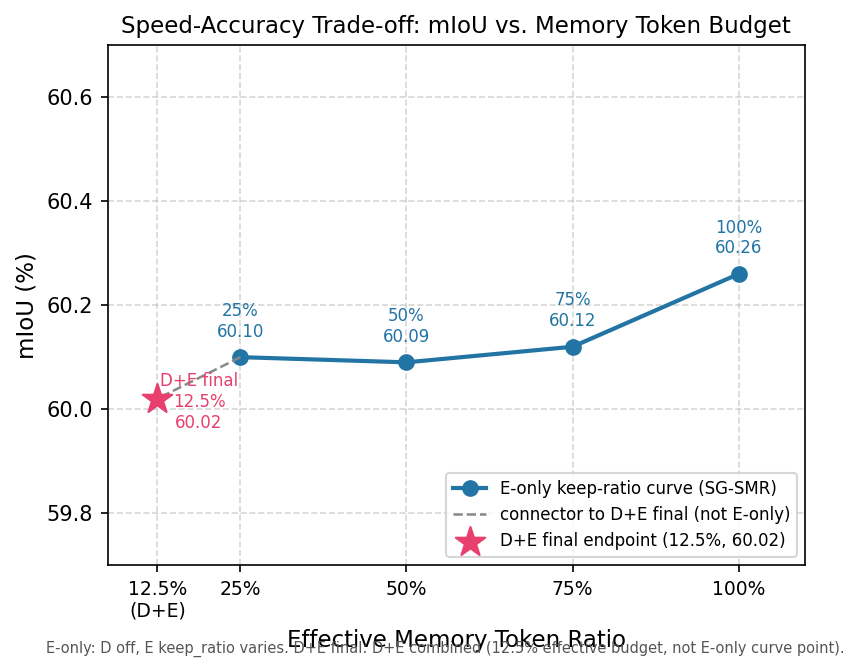
\includegraphics[width=0.78\linewidth]{figures/fig_speed_accuracy_tradeoff_miou.png}
    \caption{固定伪标签消融设置下的训练效率与 mIoU 权衡。不同配置展示了 memory token 约简所带来的效率收益及相应精度变化。该图不属于 full protocol 主结果。}
    \label{fig:speed_accuracy_tradeoff}
\end{figure}

\subsection{Token Budget}
\begin{table}[t]
  \centering
  \small
  \setlength{\tabcolsep}{3pt}
  \renewcommand{\arraystretch}{1.08}
  \caption{不同 Memory Token 预算下的精度与效率权衡。结果来自固定伪标签消融设置。}
  \label{tab:token_budget}
  \begin{tabular}{lrrrrr}
    \toprule
    Token 预算 & Tokens$\downarrow$ & mIoU$\uparrow$ & BFScore$\uparrow$ & Step (s)$\downarrow$ & Mem. Attn. (s)$\downarrow$ \\
    \midrule
    100\% & 32768 & 60.26 & 39.59 & 2.4089 & 117.56 \\
    75\% & 24576 & 60.12 & 39.28 & 2.4614 & 98.62 \\
    50\% & 16384 & 60.09 & 39.23 & 2.3798 & 79.69 \\
    25\% & 8192 & 60.10 & 39.29 & 2.2941 & 60.54 \\
    12.5\%$^{\dagger}$ & 4096 & 60.02 & 39.23 & 2.3153 & 51.92 \\
    \bottomrule
  \end{tabular}

  \vspace{0.3em}
  \footnotesize{$^{\dagger}$100\%--25\% 为仅使用稀疏检索的 Token Budget 曲线；12.5\% 为 MTC+SMR 组合端点。}
\end{table}


表~\ref{tab:token_budget} 与图~\ref{fig:token_budget_attention} 显示，Memory Attention Time 随 Token Budget 降低而整体下降，而 mIoU 与 BFScore 只在较小范围内波动。这一趋势将计算变化与有效 memory token 数直接联系起来，也表明部分历史上下文可以在不引发整体预测崩塌的情况下被约简。100\%--25\% 构成仅使用 SMR 的 Token Budget 曲线，用于比较同一稀疏检索机制的保留比例；12.5\% / 4096 tokens 是 MTC+SMR 组合端点，不能视为该曲线的自然延伸。Step Time 不严格单调，说明 top-k 选择、编码解码和数据处理等成本会共同影响单步耗时，Memory Attention Time 更适合解释 Token Budget 的直接作用。

\begin{figure}[t]
    \centering
    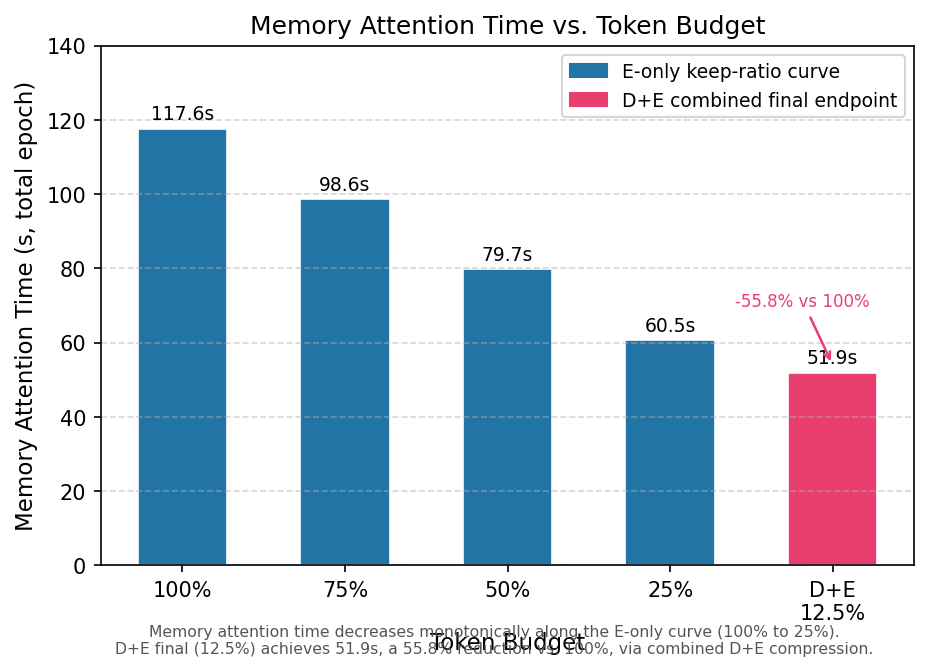
\includegraphics[width=0.78\linewidth]{figures/fig_token_budget_attention_time.png}
    \caption{固定伪标签消融设置下 Token Budget 与 Memory Attention Time 的关系。100\%--25\% 为仅使用 SMR 的曲线，12.5\% 为 MTC+SMR 组合端点。}
    \label{fig:token_budget_attention}
\end{figure}

\subsection{PQR 辅助消融}
\begin{table}[t]
  \centering
  \small
  \setlength{\tabcolsep}{4pt}
  \renewcommand{\arraystretch}{1.08}
  \caption{固定伪标签设置下的辅助伪标签质量消融。结果仅用于探索监督可靠性，不构成本文主要性能结论。}
  \label{tab:pseudo_label_ablation}
  \begin{tabular}{lccc}
    \toprule
    方法 & mIoU$\uparrow$ & 相对 R0 & 相对上一配置 \\
    \midrule
    Identity（R0） & 60.02 & -- & -- \\
    类别均衡过滤（R2） & 60.07 & +0.05 & +0.05 \\
    + 原型引导门控（R2+R4） & 60.05 & +0.03 & -0.02 \\
    \bottomrule
  \end{tabular}
\end{table}


表~\ref{tab:pseudo_label_ablation} 中，Identity、类别均衡过滤与原型引导门控的 mIoU 分别为 60.02、60.07 和 60.05。类别均衡过滤仅带来 $+0.05$，说明调整类别覆盖可能略微改善目标域监督，但变化幅度不足以支持强结论；加入原型门控后未进一步改善。一个可能原因是额外过滤减少了有效监督，或批次级原型对稀有类别和域偏移仍不稳定。由于这些解释尚未由更多诊断验证，PQR 仅作为伪标签可靠性辅助探索，不构成主要贡献。

综合消融结果，MTC+SMR 对降低 memory attention 开销的证据最直接，但更低 token budget 会增加细粒度语义与边界损失风险。模块消融解释了效率收益的来源，token budget 则界定压缩强度，PQR 仅补充监督可靠性分析；三者的实验角色不能互换。训练效率与分割质量需要共同权衡。
